\chapter{Introducción}
\label{cap1}
	A principios del siglo \emph{XX} se descubrió la existencia de los rayos cósmicos. Estos son partículas subatómicas provenientes del espacio
	exterior. Estas partículas, en su mayoría protones y núcleos de Helio, son muy energéticas debido a su gran velocidad. El origen de estas no
	está muy claro, pero sabemos que proceden del espacio exterior. Raras veces la actividad solar puede producir partículas tan energéticas. 
	\par
	Muchas de estas partículas inciden en la atmósfera terrestre. En las capas altas de la atmósfera se producen las primeras interacciones, estas
	partículas colisionan con las partículas que forman la atmósfera. Esta colisión es muy violenta y causa la división de las partículas
	originales en partículas secundarias. Estas a su vez pueden colisionar con otras partículas de la atmósfera para así formar aún más partículas
	secundarias. Vemos como una sola partícula proveniente del espacio produce el fenómeno denominado \emph{cascadas atmosféricas}. Como es de
	esperar con cada choque consecutivo se pierde parte de la energía. Normalmente las partículas secundarias que alcanzan la superficie terrestre
	tan solo tienen una pequeña fracción de la energía inicial. Si una partícula no posee la energía suficiente la cascada que es originada no se
	propaga hasta la superficie terrestre.
	\par
	Como hemos dicho la mayor parte de la radiación cósmica proviene de fuera de nuestro sistema solar, pero está fuertemente relacionada con los
	ciclos solares. Los ciclos solares de 11 años aproximadamente afectan la actividad solar pasando por un mínimo y un máximo, donde los cambios
	son apreciables en la luminosidad y el campo magnético. Es este segundo, el campo magnético solar, el que afecta a la llegada de radiación
	cósmica a la Tierra. Al ser mayormente partículas con carga eléctrica en la presencia de un fuerte campo magnético estas son desviadas. A
	continuación detallamos los sucesos más comunes que pueden ser observados indirectamente a consecuencia de estudiar la cantidad de radiación
	cósmica.
	\begin{itemize}
		\item	Ciclo solar. Como hemos explicado existe una fuerte relación entre la cantidad de radiación cósmica y la actividad solar. La
			radiación cósmica es un buen indicador de la actividad solar donde la relación es inversa. Menos radiación generalmente
			significa una actividad solar elevada.
		\item	\emph{Forbush decrease}\cite{Forbush1938}. Estos sucesos consisten en un descenso rápido de los niveles de radiación cósmica medida
			en la Tierra. Estos descensos son consecuencia de CME's(Eyección de masa coronal). La materia expulsada en un CME al ser en su
			mayoría plasma, extiende e intensifica el campo magnético solar. Como ya hemos explicado el aumento del campo magnético solar
			conlleva al descenso de radiación cósmica.
		\item	\emph{Ground level enhancements}(GLE). Eventualmente la actividad solar es tan elevada que el Sol es capaz de emitir partículas muy
			energéticas. Estas partículas son a veces tan energéticas que pueden generar cascadas atmosféricas que alcanzan la superficie
			terrestre. Estos sucesos son muy raros, entre 10 y 15 por década. A pesar de ser muy raros estos pueden tener un gran impacto
			en nuestras vidas cotidianas, pueden afectar el funcionamiento de la electrónica sensible que está en orbita e incluso la que
			está en tierra.   
	\end{itemize}

    \section{Monitor de neutrones}
        Un monitor de neutrones es una estación terrestre que monitoriza la llegada de partículas extraterrestres de forma indirecta a partir de las
        cascadas atmosféricas. Este está compuesto por cuatro capas especialmente diseñadas para capturar las partículas secundarias producidas en las
        cascadas atmosféricas. A continuación procedemos a explicar estas cuatro capas.
        \begin{itemize}
            \item	\textbf{Reflector}. La primera capa, la exterior, consiste en un escudo reflector que tan solo deja pasar las partículas con
                energía alta.  De esta manera todas las partículas generadas por el entorno inmediato que tienen baja energía rebotan y no
                influyen en la medición.
            \item	\textbf{Productor}. Esta capa compuesta generalmente de material denso tiene como objetivo conseguir algo parecido a las
                cascadas atmosféricas. La idea es tener un material denso para que aumente la probabilidad de que las partículas secundarias
                impacten con las partículas del material y como resultado se produzcan aún más partículas. A las partículas generadas en esta
                capa se les da el nombre de neutrones de evaporación. Son estas partículas las que finalmente serán medidas por el
                instrumento, también son las que le dan nombre. Los neutrones producidos tienen menos energía, por lo que son más fáciles de
                medir.
            \item	\textbf{Moderador}. A pesar de que las partículas que tenemos a este nivel tienen tan solo una fracción de la energía
                original, estas aún siguen siendo demasiado energéticas para ser capturadas. Esta capa tiene como objetivo ralentizar,
                disminuir la energía, de las partículas para así poder capturarlas.
            \item	\textbf{Contador}. Un contador proporcional o tubo contador generalmente está relleno de gas con propiedades específicas.
                Cuando el gas interacciona con los neutrones de evaporación este es ionizado, en el proceso son liberados electrones. Debido
                al campo eléctrico que atraviesa constantemente el gas estos electrones son acelerados hacia el ánodo, hilo conductor que
                atraviesa el tubo contador en su centro. Conforme los electrones ganan energía, estos pueden producir ionizaciones
                secundarias. El número total de electrones que llegan al ánodo se mantiene, sin embargo, proporcional a la energía de la
                partícula inicial. Al llegar al ánodo estos electrones producen una corriente eléctrica. 

        \end{itemize}
        \par
        Los sistemas de adquisición están diseñados para recoger estas pequeñas corrientes eléctricas y medirlas. Tradicionalmente la medida que se
        realiza son eventos por minuto, las señales son capturadas, amplificadas y registradas en un contador que se reinicia cada minuto. A lo largo
        de este trabajo muchas veces nos referiremos a esta medición de eventos por minuto con el nombre de \emph{cuentas}. 

    \section{CaLMa}
        CaLMa\cite{Medina2013} o \emph{Castilla la Mancha Neutron Monitor} es el primer y único monitor de neutrones en España. Este forma parte del
        NMDB, el equipo técnico responsable de la estación está profundamente implicado en desarrollar sistemas y herramientas que mejoran la red. Un
        ejemplo es el sistema de adquisición implantado en la estación, también implantado en otras estaciones de la red. La estación empezó a operar
        de forma plena en diciembre de 2012 y desde entonces lleva haciéndolo ininterrumpidamente con pequeñas excepciones. Desde su puesta en marcha
        la estación ha registrado 18 Forbush decreases. Desafortunadamente aún no ha habido ningún GLE que detectar, aunque este tendría que ser muy
        energético para ser detectado en una estación con tan poca latitud.

    \section{Proceso de adquisición}
        El propósito de este punto es explicar algunos aspectos del proceso de
        adquisición que son relevantes para este trabajo.
        \par
        Hasta este momento siempre hemos hablado de tubos contadores, en plural,
        detrás de esto hay una razón. Normalmente las estaciones se componen de
        varios tubos contadores, donde 18 tubos contadores es un estándar. En el
        proceso de adquisición están envueltos muchos factores probabilísticos,
        esto conlleva a que las medidas en un tubo tengan una gran dispersión. La
        solución de este problema es tener muchos tubos, cuantos más mejor.
        Combinando datos de diferentes tubos conseguimos reducir esta dispersión. 
        \par
        Tener los datos de muchos tubos contadores permite reducir la dispersión de
        los datos, sin embargo no es muy práctico trabajar con esos datos en crudo.
        El software del sistema de adquisición actual calcula un valor global a
        partir de los datos de todos los tubos contadores, para este propósito es
        utilizado el Median Algorithm\cite{MedianAlgr}.
        \par
        Anteriormente en este capítulo explicamos las cascadas atmosféricas que son
        originadas por los rayos cósmicos. Estas cascadas atmosféricas dependen de
        la presión atmosférica. Cuando esta es elevada, son necesarias particulas
        con más energía para que la cascada se propague hasta el nivel terrestre,
        por consecuente los monitores de neutrones registran menos eventos. El
        valor de la presión atmosférica es monitorizado por los monitores de
        neutrones. Este valor es utilizado para realizar una corrección por presión
        sobre el valor global de la estación, a lo largo de este trabajo utilizamos
        el término de \emph{valor corregido por presión} para referirnos a este
        valor.
        \par
        También es realizada una \emph{corrección por eficiencia}. Esta es muy
        simple y consiste en aplicar un factor multiplicativo al \emph{valor
        corregido por presión}. Este valor es utilizado para para solventar
        problemas técnicos. Cambios en el entorno inmediato del instrumento o
        cambios en la electrónica utilizada pueden afectan a la cantidad de eventos
        medidos. Estos cambios son identificados, evaluados y finalmente
        contrarrestados con esta corrección por eficiencia. Este valor dota la
        estación de consistencia histórica, de esta manera pueden ser comparados
        datos de diferentes intervalos temporales.
        \par
        Al principio de este capítulo explicamos que los tubos contadores están
        rellenos de gas con propiedades especiales. Sobre este gas es aplicado un
        campo eléctrico. Para la generación de dicho campo son utilizadas fuentes
        de alimentación de alta tensión. Cambios en la tensión generada pueden
        afectar a la cantidad de eventos registrados. Esto ha conllevado a que el
        funcionamiento de las fuentes sea monitorizado. El software para el sistema
        de adquisición debe ser capaz de realizar esta operación. Es de esperar que
        la tensión sea constante, en caso de variaciones los datos generados son
        considerados no consistentes.








\chapter{Sistema de adquisición}
\label{cap2}
    \section{Introducción}
        Como hemos mencionado el sistema de adquisición que está implantado en
        CaLMa es producto del propio equipo\cite{Garcia2014}. Este está basado en
        un sistema empotrado Linux. Si las señales generadas por los tubos
        contadores superan un determinado umbral, estas son covertidas en pulsos
        digitales por los amplificadores. A continuación, un circuito de adaptación
        se encarga de elevar los niveles de tensión de los pulsos digitales a
        niveles \emph{TTL} y de adaptar la impedancia de la línea de comunicaciones
        si el amplificador así lo requiere. Seguidamente los pulsos son procesados
        por una FPGA que es la encargada de medir los eventos por minuto de los 18
        canales. Aunque la estación tan solo tiene 15 tubos contadores el sistema
        está diseñado para soportar 18, este número es un estándar histórico. El
        software que se ejecuta en el sistema Linux tiene como tarea comunicarse
        con la FPGA, el barómetros y las fuentes de alimentación. La labor de este
        es recoger la información de los demas dispositivos, procesarla y
        finalmente guardar esta en una base de datos. El software hace uso del
        \emph{Network Time Protocol} para asegurar la correcta sincronización
        temporal entre estaciones, esta sincronización permite contrastar los datos
        de diferentes estaciones. En la figura \ref{fig:acqsis} podemos ver un
        diagrama de bloques que representa el sistema de adquisición.
        \begin{figure}[h]
            \centering
            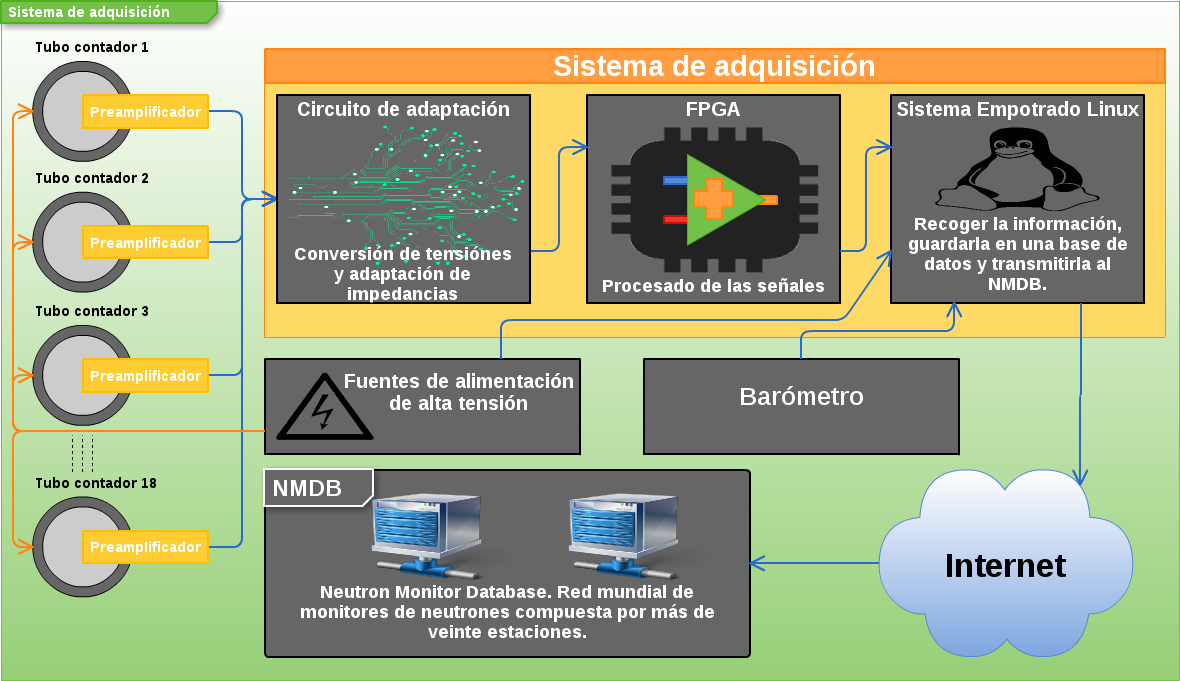
\includegraphics[keepaspectratio, width=1\textwidth]{./img/AcqSis.png}
            \caption{Sistema de adquisición.}
            \label{fig:acqsis}
        \end{figure}

    \section{BeagleBone Black}
        \emph{BeagleBone Black}\cite{Beagle}\cite{BeagleWiki} es un computador
        empotrado, \emph{open-source} y \emph{single board}. La placa viene con
        Linux, distribución \emph{Angstrom} y versión de núcleo 3.8. En la
        figura \ref{fig:beaglebone} podemos ver un diagrama de bloques que
        refleja los componentes hardware que componen la \emph{BeagleBone
        Black}. A continuación vamos a hacer una breve descripción de los
        módulos utilizados en el sistema de adquisición.
        \begin{itemize}
            \item 	ARM CORTEX A8\cite{BeagleCore} y SDRAM. El procesador y los
                512MB DRR3 de memoria RAM son suficientementes para soportar la
                distribución Linux y satisfacer las necesidades del software.
            \item 	Ethernet Connector. El conector RJ-45 permite establecer
                una conexión a Internet. Una vez establecida esta conexión los
                datos pueden ser transmitidos al NMDB. También es posible
                establecer una conexión a la placa vía SSH, de esta manera un
                operador puede realizar operaciones de mantenimiento de forma
                remota.
            \item	eMMC y microSD. Utilizamos la memoria integrada (eMMC) de
                4GB para albergar el sistema operativo y el software de
                adquisición. La microSD es utilizada para guardar los datos y
                logs producidos por el software de adquisición.
            \item 	Analog Pins. Los 7 pines analógicos permiten usar sensores
                cuyo output es una señal analógica. Ejemplo de estos sensores
                son las fuentes de alimentación analógicas o los sensores de
                temperatura, en algunas estaciones la temperatura ambiente se
                monitoriza también. Estos sensores producen señales cuya
                tensión eléctrica es proporcional al valor de la magnitud
                medida. 
            \item 	GPIOs. Los \emph{General Purpose Input/Output} permiten
                trabajar con señales digitales, tanto de entrada como de
                salida. Un ejemplo de uso es la señal de Reset de la FPGA,
                señal digital activa a bajo nivel.
            \item	UARTs. La placa ofrece 4 puertos serie de los que
                utilizamos 2 para comunicarnos con la FPGA.
        \end{itemize}
        \begin{figure}[h]
            \centering
            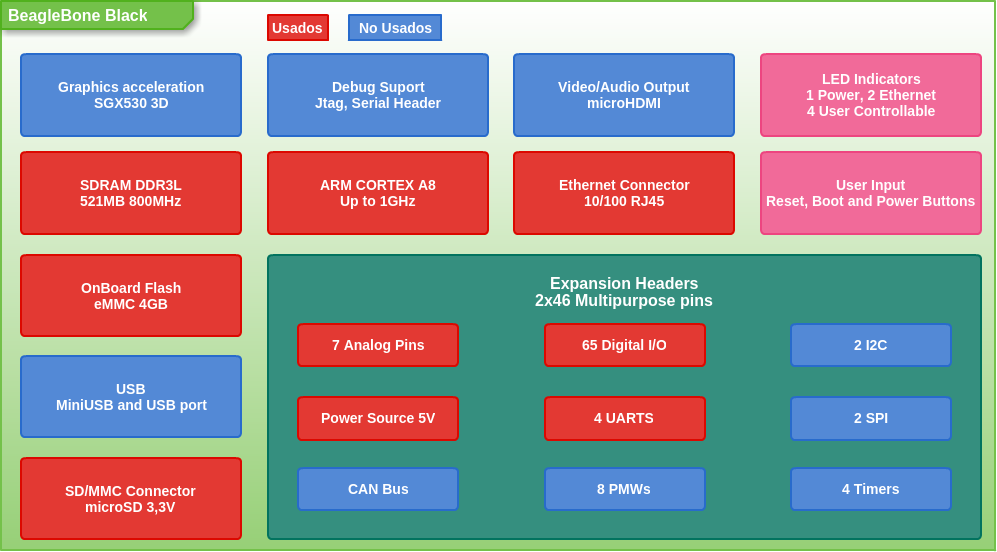
\includegraphics[keepaspectratio, width=1\textwidth]{./img/beaglebone.png}
            \caption{\emph{BeagleBone Black}. Diagrama de bloques hardware}
            \label{fig:beaglebone}
        \end{figure}
        \par
        Fijándonos en la figura \ref{fig:beaglebone} podemos ver que muchos de
        los módulos son accesibles mediante los conectores de
        expansión\cite{BeagleWikiExp}. Estos conectores tienen 2x46 pines, de
        los cuales muchos son multipropósito. Estos pueden ser configurados
        para tener funcionalidades diversas y además esta configuración puede
        ser realizada de forma dinámica. La configuración de los pines se
        realiza mediante el \emph{Device Tree Overlay}, estructura de datos que
        se utiliza para describir el hardware. En la realización del software
        no lidiamos con este mecanismo, sino que se utiliza una biblioteca que
        facilita el trabajo. La biblioteca utilizada es \emph{Adafruit
        BeagleBone IO Python}\cite{AdaFruitGit}. Esta ayuda a configurar
        dinámicamente los pines de expansión, además ofrece métodos para operar
        sobre estos una vez configurados.

    \section{FPGA}
        La FPGA es el núcleo fundamental del sistema, ya que se encarga de procesar las señales y de transmitir la información al software de
        adquisición. Una FPGA es un circuito integrado formado por unidades lógicas cuya interconexión y funcionalidad pueden ser configurados
        mediante un lenguaje de descripción de hardware, típicamente \emph{Verilog} o \emph{VHDL}. Esta configuración del hardware de la FPGA, también
        conocida como \emph{IP core}, es la que establece la funcionalidad de una FPGA. En esta sección vamos a hacer una descripción funcional de la
        FPGA, y por consiguiente se describirá el \emph{IP core} de la misma. En la figura \ref{fig:fpga} podemos ver un diagrama de bloques que
        refleja los módulos e interfaces que el \emph{IP core} posee.
        \begin{figure}[h]
            \centering
            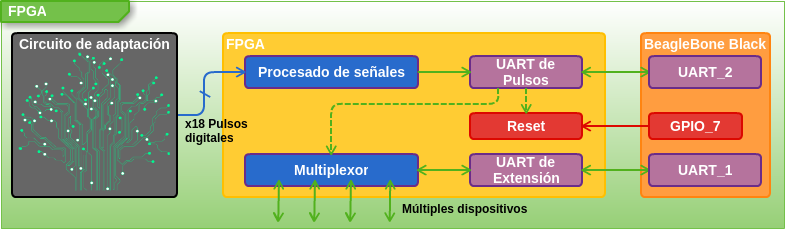
\includegraphics[keepaspectratio, width=1\textwidth]{./img/fpga.png}
            \caption{FPGA. Diagrama de bloques.}
            \label{fig:fpga}
        \end{figure}	
        \subsection{Procesado de pulsos}
            Como hemos comentado la FPGA es la encargada de procesar las señales y trasmitir la información a la \emph{BeagleBone Black}. Esta
            transmisión se realiza mediante una línea serie asíncrona de 1Mbps. La línea está controlada por una UART(\emph{Universal Asynchronous
            Receiver-Transmitter}) a la que nos referiremos como \emph{UART de pulsos}. En las tablas \ref{tab:FPGAUartPulso},
            \ref{tab:FPGAUartOver} y \ref{tab:FPGAUartCont} podemos ver el formato de los datos transmitidos. Vemos que hay tres mensajes
            diferentes que la FPGA puede transmitir.
            \begin{itemize}
                \item	En la tabla \ref{tab:FPGAUartPulso} podemos ver el formato del primer mensaje que vamos a discutir. Este mensaje se
                    compone de tres bytes que dan información sobre el ancho de un pulso. El mensaje permite identificar el canal en el
                    que se ha producido el pulso, el nivel (alto/bajo) y la longitud de este. Los pulsos de nivel alto representan la
                    detección de una partícula por los tubos contadores y el ancho del pulso es proporcional a la energía de la partícula
                    detectada. La longitud de los pulsos de nivel bajo también se mide para poder identificar pulsos con pequeña
                    separación temporal, que podrían indicar la presencia de un fenómeno físico denominado multiplicidad.
                \item 	En la siguiente tabla \ref{tab:FPGAUartOver} podemos apreciar el mensaje de estado que la FPGA genera. Dado que la UART usa
                    una FIFO de tamaño fijo es posible que la esta se llene y se pierdan mensajes. En este caso se genera un mensaje de
                    estado que es transmitido para indicarle al software que se han producido perdidas de datos.
                \item	Además de medir el ancho de los pulsos la FPGA lleva la cuenta de pulsos recibidos para cada canal. Esta información
                    puede ser solicitada por la \emph{BeagleBone Black} utilizando el comando apropiado(ver tabla \ref{tab:FPGAUartComm}). En la
                    tabla \ref{tab:FPGAUartCont} podemos ver el formato en el que se transmite la información de las cuentas. Los bytes 2,
                    3 y 4 son transmitidos 18 veces, una vez para cada canal. Después de transmitir la información de las cuentas la FPGA
                    reinicia los contadores para cada canal.
            \end{itemize}
            En la figura \ref{fig:fpgaWave} podemos observar un ejemplo de la secuencia de datos transmitidos por la \emph{UART de pulsos}, junto a
            estos podemos apreciar los estímulos que los causan. 

            \begin{table}[h]
                \tiny
                \begin{tabularx}{\textwidth}{|l|c|c|X|c|c|c|c|c|}
                    \hline
                    \rowcolor[HTML]{C0C0C0} 
                    \multicolumn{1}{|r|}{\textbf{Bit}}    	& 7 & 6          & 5 				& 4 	       & 3 	     & 2 	  & 1          & 0 	     \\ \hline
                    \cellcolor[HTML]{C0C0C0}\textbf{Byte 1} & 0 & 1          & 0  				& \multicolumn{5}{c|}{Canal (0-17)}				     \\ \hline
                    \cellcolor[HTML]{C0C0C0}\textbf{Byte 2} & 1 & Dato (6)	 & Dato (5)      		& Dato (4)     & Dato (3)    & Dato (2)   & Dato (1)   & Dato (0)    \\ \hline
                    \cellcolor[HTML]{C0C0C0}\textbf{Byte 3} & 1 & X          & Nivel ('1'->alto, '0'->bajo) & Dato (11)    & Dato (10)   & Dato (9)   & Dato (8)   & Dato (7)    \\ \hline
                \end{tabularx}
                \caption{\emph{UART de pulsos}. Palabra de ancho de pulso}
                \label{tab:FPGAUartPulso}
                \begin{tabularx}{\textwidth}{|l|c|X|X|X|X|X|X|X|}
                    \hline
                    \rowcolor[HTML]{C0C0C0} 
                    \multicolumn{1}{|r|}{\textbf{Bit}} 	& 7 & 6 		       & 5 		       & 4		       & 3 		       & 2		       & 1          	       & 0			\\ \hline
                    \cellcolor[HTML]{C0C0C0}\textbf{Byte 1} & 0 & 0                        & OverFlow FIFO Tubo 5  & OverFlow FIFO Tubo 4  & OverFlow FIFO Tubo 3  & OverFlow FIFO Tubo 2  & OverFlow FIFO Tubo 1  & OverFlow FIFO Tubo 0	\\ \hline
                    \cellcolor[HTML]{C0C0C0}\textbf{Byte 2} & 1 & OverFlow FIFO Tubo 12    & OverFlow FIFO Tubo 11 & OverFlow FIFO Tubo 10 & OverFlow FIFO Tubo 9  & OverFlow FIFO Tubo 8  & OverFlow FIFO Tubo 7  & OverFlow FIFO Tubo 6	\\ \hline
                    \cellcolor[HTML]{C0C0C0}\textbf{Byte 3} & 1 & Almost Full FIFO General & OverFlow FIFO General & OverFlow FIFO Tubo 17 & OverFlow FIFO Tubo 16 & OverFlow FIFO Tubo 15 & OverFlow FIFO Tubo 14 & OverFlow FIFO Tubo 13	\\ \hline
                \end{tabularx}
                \caption{\emph{UART de pulsos}. Palabra de estado}
                \label{tab:FPGAUartOver}
                \begin{tabularx}{\textwidth}{|l|X|c|c|c|c|c|c|c|}
                    \hline
                    \rowcolor[HTML]{C0C0C0} 
                    \multicolumn{1}{|r|}{\textbf{Bit}}    	 & 7 & 6           & 5 		& 4 	      & 3 	    & 2 	 & 1           & 0 	     	\\ \hline
                    \cellcolor[HTML]{C0C0C0}\textbf{Byte 1}  & 0 & 1           & 1  	& X	      & X	    & X	  	 & X	       & X	     	\\ \hline
                    \cellcolor[HTML]{C0C0C0}\textbf{Byte 2}  & 1 & Dato0 (6)   & Dato0 (5) 	& Dato0 (4)   & Dato0 (3)   & Dato0 (2)  & Dato0 (1)   & Dato0 (0)  	\\ \hline
                    \cellcolor[HTML]{C0C0C0}\textbf{Byte 3}  & 1 & Dato0 (13)  & Dato0 (12)	& Dato0 (11)  & Dato0 (10)  & Dato0 (9)  & Dato0 (8)   & Dato0 (7)  	\\ \hline
                    \cellcolor[HTML]{C0C0C0}\textbf{Byte 4}  & 1 & X	   & X	 	& X	      & X	    & X		 & Dato0 (15)  & Dato0 (14)	\\ \hline
                    \cellcolor[HTML]{C0C0C0}\textbf{Byte 5}  & 1 & Dato1 (6)   & Dato1 (5) 	& Dato1 (4)   & Dato1 (3)   & Dato1 (2)  & Dato1 (1)   & Dato1 (0)  	\\ \hline
                    \cellcolor[HTML]{C0C0C0}\textbf{......}  & . & .........   & ......... 	& .........   & .........   & .........  & .........   & .........  	\\ \hline
                    \cellcolor[HTML]{C0C0C0}\textbf{Byte 55} & 1 & X	   & X	 	& X	      & X	    & X		 & Dato17 (15) & Dato17 (14)	\\ \hline
                \end{tabularx}
                \caption{\emph{UART de pulsos}. Palabra de cuentas}
                \label{tab:FPGAUartCont}
                \begin{tabularx}{\hsize}{|c|X|}
                    \hline
                    \rowcolor[HTML]{C0C0C0} 
                    Commando & Descripción                            \\\hline
                    0x00     & Configura multiplexor para aparato 1   \\\hline
                    0x01     & Configura multiplexor para aparato 2   \\\hline
                    0x02     & Configura multiplexor para aparato 3   \\\hline
                    0x03     & Configura multiplexor para aparato 4   \\\hline
                    0x10     & Reset general del sistema              \\\hline
                    0x11     & Solicita la transmisión de las cuentas \\\hline
                \end{tabularx}
                \caption{\emph{UART de pulsos}. Commandos}
                \label{tab:FPGAUartComm}
            \end{table}
            \begin{figure}[h]
                \centering
                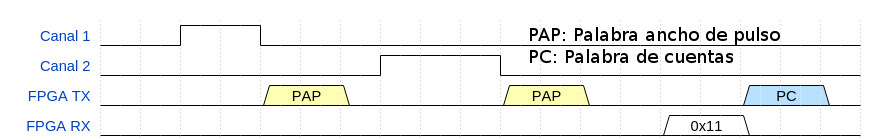
\includegraphics[keepaspectratio, width=1\textwidth]{./img/fpgawave.png}
                \caption{FPGA. Diagrama de eventos.}
                \label{fig:fpgaWave}
            \end{figure}
        \subsection{Multiplexor}
            Tal y como explicamos en el capítulo de introducción, el sistema de adquisición debe monitorizar la presión atmosférica, el
            funcionamiento de las fuentes de tensión y en muchos casos la temperatura ambiente. Al igual que muchos otros dispositivos que pueden
            ser necesarios, la mayoría de estos sensores hacen uso de un puerto serie. Estos son manejados según el patron \emph{Master-Slave} y
            generalmente intercambian poca información, por consiguiente, pueden compartir un puerto serie. El mecanismo que resuelve este
            problema está implmentado en el \emph{IP core}. Este consiste en una UART a la que nos referiremos como \emph{UART de extensión}. Esta
            está conectada a un multiplexor, que es el encargado de realizar la conmutación entre los cuatro dispositivos soportados. El estado
            del multiplexor puede cambiarse enviando comandos por la \emph{UART de pulsos}, de acuerdo a la especificación presentada en la tabla
            \ref{tab:FPGAUartComm}. Ejemplo de dispositivos que requiren un puerto serie son el barómetro \emph{BM35} utilizado en CaLMa, varias
            fuentes de alimentación comerciales, estaciones meteorológicas, GPS, etc.
        \subsection{Reset}
            \enlargethispage{2\baselineskip}
            El \emph{IP core} permite realizar un \emph{Reset} del estado interno de la FPGA. Todas las variables son puestas a sus valores iniciales,
            excepto el multiplexor que mantiene su estado. Para la realización de dicho Reset son exportadas tres interfaces. La primera es un
            boton hardware accesible de forma física. La segunda es un commando trasmitido por la \emph{UART de pulsos}, de acuerdo a la
            especificación presentada en la tabla \ref{tab:FPGAUartComm}. Finalmente, la tercera es una señal digital activa a bajo nivel. Dicha
            señal definida como \emph{BS1}, está conectada al pin \emph{P9\_42(GPIO\_7)} de la \emph{BeagleBone Black}, por consiguiente, es accesible
            desde el software de adquisición.

\chapter{Software de adquisición}
\label{cap3}
    En este capítulo procedemos a explicar el funcionamiento del software de
    adquisición. El funcionamiento nominal del software consiste en recoger la
    información de los módulos hardware como la FPGA, el barómetro, las fuentes
    de alimentación y los sensores de temperatura si estos están presentes.
    Cada minuto, la información recogida es procesada y almacenada en una base
    de datos. 
    \par
    El software es ejecutado en la \emph{BeagleBone Black} sobre un Linux,
    distribución \emph{Angstrom}, recientemente adaptado para soportar también
    Debian. El lenguaje elegido para el desarrollo es
    \emph{Python}\cite{Python}. Este es un lenguaje interpretado de alto nivel
    con una sintaxis centrada en producir un código legible. El lenguaje se
    adapta igualmente bien a programación imperativa y orientada a objetos. El
    tipado dinámico da mucha flexibilidad al lenguaje. Todas estas propiedades
    del lenguaje permiten un desarrollo rápido. Además el lenguaje ofrece una
    amplia cantidad de bibliotecas que también aligeran el trabajo. 
    \par
    Para gestionar la base de datos se utiliza \emph{Sqlite3}\cite{Sqlite}.
    Este es un gestor muy ligero y adecuado para sistemas empotrados. Aparte de
    esta base de datos local, el software permite mantener una segunda réplica
    remota. Para esta réplica remota se utiliza \emph{MySql}\cite{MySql} que es
    un gestor más completo con enfoque \emph{Cliente-Servidor}.
    \par
    En la figura \ref{fig:soft_adquisición} podemos ver un diagrama de flujo
    que describe el funcionamiento del software. Podemos ver que hay cuatro
    módulos principales, a continuación hacemos una breve descripción de estos. 
    \begin{itemize}
        \item	\texttt{NMDA}. Es el proceso principal de nuestro software. Es
            el encargado de realizar las configuraciones necesarias e iniciar
            el \texttt{FPGASerialReader} y el \texttt{CountsManager}.
        \item	\texttt{FPGASerialReader}. \emph{Thread} que se encarga de
            procesar la información transmitida por la FPGA.
        \item	\texttt{CountsManager}. \emph{Thread} que se enarga de pedir la
            información necesaria y guardarla en la base de datos con
            periodicidad de un minuto. Después de guardar la información es
            iniciado el \texttt{DBUpdater}.
        \item	\texttt{DBUpdater}. \emph{Thread} que se encarga de sincronizar la base de datos local con la réplica remota.
    \end{itemize}
    \begin{sidewaysfigure}[p]
        \centering
        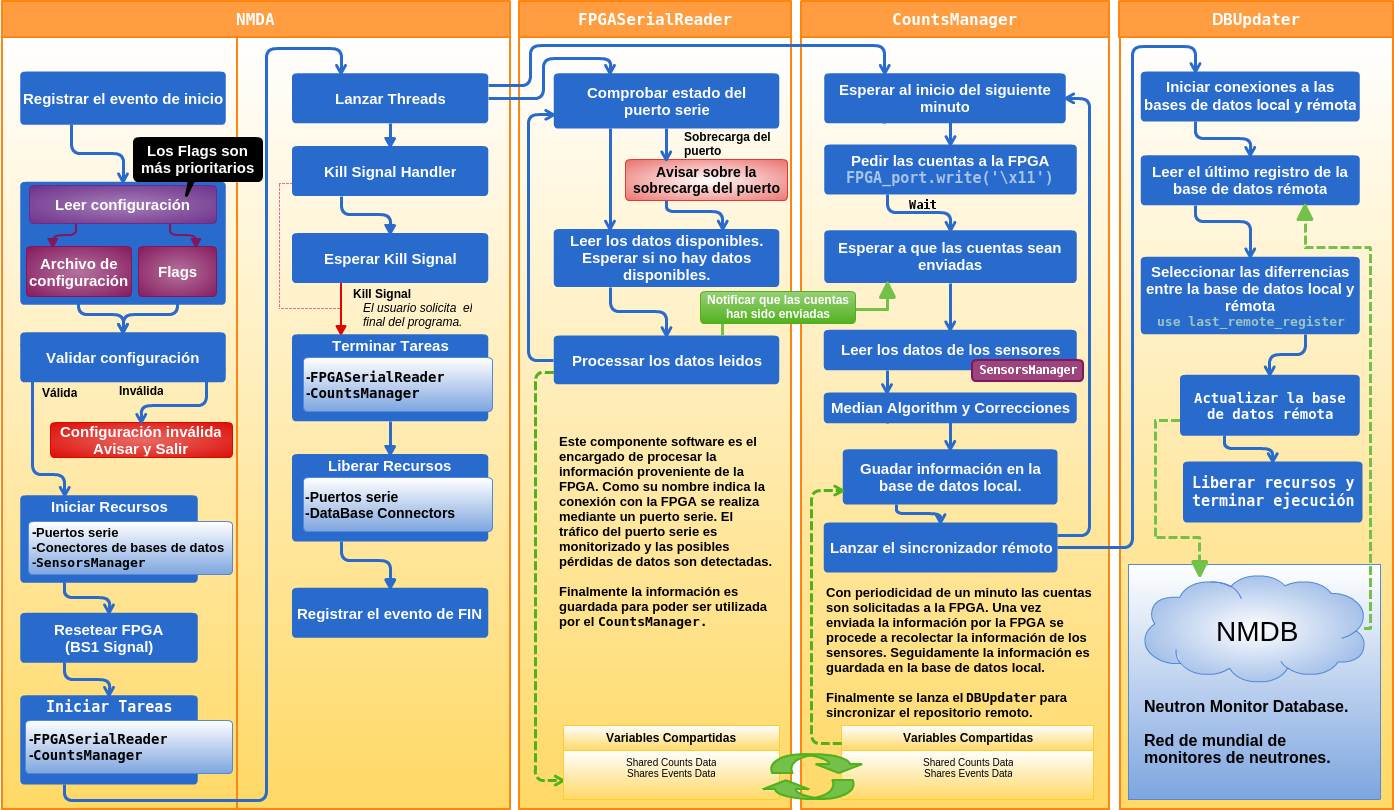
\includegraphics[keepaspectratio, width=1\textwidth]{./img/soft_adquisicion.png}
        \caption{Diagrama de flujo. Software de adquisición.}
        \label{fig:soft_adquisición}
    \end{sidewaysfigure}

    \section{Arranque automático del sistema}
        Uno de los requisitos del sistema es el arranque automático ante la presencia de corriente eléctrica. La \emph{BeagleBone Black} por defecto está
        configurada para arrancar automáticamente,pero debemos configurarla para que también inicialice nuestro software. Para este propósito vamos a
        utilizar las \emph{System Services}\cite{AngSystemctl} que \emph{Angstrom} proporciona. Esta distribución utiliza \texttt{systemd}\cite{systemdWiki}
        para gestionar los servicios de sistema y la forma en la que estos servicios arrancan cuando se pone en marcha la \emph{BeagleBone Black}. Este es un
        conjunto de demonios, bibliotecas y utilidades diseñados para facilitar la administración de sistemas Linux.
        \par
        En la figura \ref{fig:boot} podemos ver la secuencia que define el proceso de arranque del sistema de adquisición. Esta secuencia empieza con
        el servicio \texttt{myWatchDog.service}, que es el encargado de arrancar el software que controla el \emph{Watchdog}. El servicio
        \texttt{ntpdate.service} es el responsable de establecer la fecha y hora actuales mientras que el servicio \texttt{ntpd.service} tiene como
        tarea corregir las derivas que pueden presentrase. Finalmente el servicio \texttt{nmda.service} es el encargado de arrancar el software de
        adquisición.
        \begin{figure}[h]
            \centering
            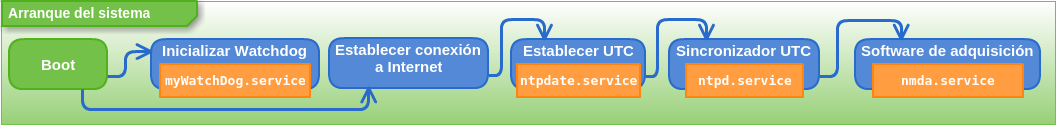
\includegraphics[keepaspectratio, width=1\textwidth]{./img/boot.png}
            \caption{Arranque del sistema}   
            \label{fig:boot}
        \end{figure}

    \section{Watchdog}
        Un \emph{Watchdog} \cite{WatchDogWiki} es un mecanismo de seguridad
        que realiza un \emph{Reset} en el sistema cuando es detectado un
        mal funcionamiento. Consiste en un temporizador que realiza una
        cuenta atrás, de forma que, cuando esta cuenta llega a cero, el
        sistema es reiniciado. Es el software el que debe reponer el valor
        de este contador para evitar que expire. Los \emph{Watchdogs}
        pueden ser software o hardware, el utilizado en este trabajo está
        implementado en la \emph{BeagleBone Black} y es hardware. Los
        \emph{Watchdogs} hardware son más fiables, los software son más
        susceptibles a bloquearse.
        \par
        El \emph{Watchdog} es accesible mediante el archivo
        \texttt{/dev/watchdog}. Para activar el mecanismo basta con
        escribir cualquier valor en dicho archivo. El contador se pone en
        marcha automáticamente y, si este llegara a expirar, se produciría
        el reinicio del sistema. El valor inicial del contador es de 60
        segundos, valor que adquiere cada vez que es reiniciado. El
        contador es reiniciado al volver a escribir en el archivo. Al
        cerrar dicho archivo el mecanismo es deshabilitado.
        \par 
        La condición que el software, encargado de reiniciar el
        \emph{Watchdog}, controla es la presencia de datos en la base de
        datos. Si el sistema no ha generado datos en los últimos 5 minutos,
        el \emph{Watchdog} deja de reiniciarse con el fin de que expire y
        cause el reinicio del sistema.

    \section{Sincronización de fecha y hoara}
        La \emph{BeagleBone Black} no implementa ningún mecanismo hardware
        para mantener la fecha y hora actuales, por lo que en cada reinicio
        la fecha y hora se pierden. Para aseguarar la correcta
        sincronización con el resto del mundo es utilizado el programa
        \texttt{ntpd}. Este programa hace uso del \emph{Network Time
        Protocol}\cite{ntpWiki}, que permite la sincronización entre dos
        relojes a través de una red de datos con latencia variable. Son
        realizadas dos llamadas a este programa.
        \begin{lstlisting}[style=myBash]
# Establece inicialmente la fecha y hora.
$ /usr/bin/ntpd -q -g -x
# Lanza un demonio que corrige las derivas que puedan presentarse
$ /usr/bin/ntpd -p /run/ntpd.pid
        \end{lstlisting}

    \section{\texttt{NMDA}}
        Este es el módulo principal del software de adquisición. Es el encargado de realizar la configuración inicial de acuerdo con los parámetros
        proporcionados, resetear la FPGA y finalmente inicializar los demás módulos. En la figura \ref{fig:soft_adquisición} podemos ver un diagrama
        de flujo que representa el funcionamiento de este. En las siguientes subsecciones describiremos las funcionalidades más relevantes de este
        módulo.
        \subsection{Logger}
            Haciendo uso de la biblioteca \texttt{logging}\cite{py_logging} se
            configura un archivo de Log. En este archivo se registran los
            sucesos de eventos importantes. El mecanismo está configurado para
            que automáticamente se guarde la hora y fecha de cada mensaje.
        \subsection{Archivo de configuración y Flags}
            Existen una serie de parámetros que varían en función de la
            estación o que simplemente pueden cambiar con el tiempo. No es
            buena idea tener los valores de estas variables en el código. Este
            problema nos ha llevado a exportar estos parámetros a un archivo de
            configuración.
            \par
            Los valores de los parámetros exportados son también accesibles a
            través de flags. Los valores especificados mediante flags tienen
            precedencia sobre los mismos que estuvieran en el archivo de
            configuración.
            \begin{lstlisting}[style=myBash]
$ python NMDA.py -h
usage: NMDA.py 
   [-h] [-sp SERIAL_PORT_CONTROL] [-db DATABASE]
   [-sps SERIAL_PORT_SENSORS] [-bm {ap1,bm35}]
   [-hv {digital,analog}] [-ahvc ANALOG_HVPS_CORR]
   [-dbU DB_UPDATER_ENABLED] [-ldb LOCAL_DB] [-rh REMOTE_DB_HOST]
   [-ru REMOTE_DB_USER] [-rp REMOTE_DB_PASS] [-rdb REMOTE_DB_DB]
   [-apr AVG_PRESSURE]
            \end{lstlisting}

        \subsection{Configurar la BeagleBone Black}
            Tal y como explicamos en el capítulo de entorno hardware la
            \emph{BeagleBone Black} proporciona dos conectores de expansión de
            46 pines cada uno\cite{BeagleWikiExp}. Muchos de estos pines son
            multipropósito, es decir, que están compartidos por varias unidades
            funcionales internas, por lo que debe configurarse a cuál de ellas
            se conectará. Esta configuración se realiza mediante el uso de
            \emph{Device Tree Overlay}, que es una estructura de datos
            utilizada para describir el hardware.
            \par
            Para el desarrollo del software de adquisición es utilizada la
            biblioteca \emph{Adafruit BeagleBone IO Python}\cite{AdaFruitGit}
            que facilita la tarea de configurar estas cabeceras. A continuación
            podemos ver una lista de los pines utilizados y la función de cada
            uno en el ámbito de este proyecto.
            \begin{lstlisting}[style=myBash]
Pin P9_21(UART2_TXD) --> Uart de Control trasmisión
Pin P9_22(UART2_RXD) --> Uart de Control recepción
Pin P9_24(UART1_TXD) --> Uart de Extensión trasmisión
Pin P9_26(UART1_RXD) --> Uart de Extensión recepción
Pin P9_37(AIN2)	     --> Entrada analógica(sensores analógicos)
Pin P9_38(AIN3)	     --> Entrada analógica(sensores analógicos)
Pin P9_39(AIN0)	     --> Entrada analógica(sensores analógicos)
Pin P9_40(AIN1)	     --> Entrada analógica(sensores analógicos)
Pin P9_42(GPIO_7)    --> Reset de la FPGA.
Pin P8_08(GPIO_67)   --> Señal DATA del barómetro AP1.
Pin P8_09(GPIO_69)   --> Señal CLOCK del barómetro AP1.
Pin P8_10(GPIO_68)   --> Señal STROBE del barómetro AP1.
            \end{lstlisting}

        \subsection{Iniciar recursos}
            Al ser el módulo principal, \texttt{NMDA} es el encargado de
            iniciar todos los recursos que serán utilizados. Por recursos nos
            referimos a las variables compartidas entre \emph{threads},
            conectores a las bases de datos, interfaces de los puertos serie y
            otros. Para los conectores a las bases de datos son utilizadas las
            bibliotecas \texttt{sqlite3} y \texttt{MySQLdb}, volvemos a
            recordar que tenemos una réplica local con \emph{Sqlite3} y otra
            réplica remota que gestionamos con \emph{MySql}. Las tablas son
            creadas automáticamente en caso de no existir, esto simplifica
            mucho el proceso de implantación. Para la interfaz de los puertos
            serie es utilizada la biblioteca \texttt{serial}.
            \par
            Son inicializados los otros dos \emph{threads},
            \texttt{FPGASerialReader} y \texttt{CountsManager}. Estos dos
            realizan todo el proceso de adquisición y serán descritos más
            adelante en este capítulo. 
        \subsection{Resetear FPGA}
            Como hemos explicado en el capítulo \ref{cap2}, la FPGA
            permite realizar un \emph{Reset}, que el software realizará antes
            de empezar con la adquisición de datos. Este \emph{Reset} asegura
            que la FPGA está en un correcto estado. Para realizar el
            \emph{Reset} utilizamos la señal digital, \emph{BS1}, que está
            conectada al pin \emph{P9\_42} de la \emph{BeagleBone Black}.
            Volvemos a recordar que esta es activa a nivel bajo. Para
            controlarla utilizaremos la biblioteca de
            \emph{AdaFruit}\cite{AdaFruitGit}, que gestiona las entradas y
            salidas de propósito general(GPIO) de la siguiente forma.
            \begin{lstlisting}[style=myPython]
import Adafruit_BBIO.GPIO as GPIO
GPIO.setup('P9_42', GPIO.OUT)
GPIO.output('P9_42', GPIO.LOW)
time.sleep(0.5)
GPIO.output('P9_42', GPIO.HIGH)
            \end{lstlisting}

    \section{\texttt{FPGASerialReader}}
        Este módulo software es el encargado de leer y procesar los datos
        transmitidos por la FPGA. En la figura \ref{fig:soft_adquisición}
        podemos ver un diagrama de flujo que refleja el funcionamiento de este.
        La ejecución del \emph{thread} empieza comprobando el estado del puerto
        serie, que puede estar saturándose. En el caso de que el puerto esté
        saturado se genera una entrada en el archivo de Log indicando este
        hecho. A continuación leemos los datos disponibles, y en caso de no
        haber datos disponibles el \emph{thread} se queda bloqueado esperando a
        la llegada de estos. Seguidamente de leer los datos pasamos a
        procesarlos. Por procesar nos referimos a interpretar el significado
        que tienen. Finalmente volvemos al paso inicial, volviendo a comprobar
        si han llegado nuevos datos a la UART.
        \par
        En las tablas \ref{tab:FPGAUartPulso}, \ref{tab:FPGAUartOver} y
        \ref{tab:FPGAUartCont}  del capítulo \ref{cap2}, podemos ver el
        formato de los datos que tenemos que procesar. Vemos que hay tres tipos
        de mensajes que podemos recibir. Los mensajes no siguen un orden
        concreto, además llegan de forma totalmente asíncrona. Además el canal
        de trasmisión no asegura la correcta trasmisión de los bytes por lo que
        algunos pueden perderse. Todo esto conlleva a que procesar los datos no
        sea una tarea fácil.
        \par
        Para solucionar este problema hemos implementado una máquina de Moore.
        Si nos volvemos a fijar en el formato de los datos podemos ver que los
        primeros bits de cada byte son fijos. Estos bits ayudan a identificar a
        que mensaje corresponde el byte. Los estados y transiciones de la
        máquina pueden verse en la figura \ref{fig:reader}. El estado inicial
        es \texttt{ByteX}. Aunque no esté reflejado en la figura la recepción
        de cualquier valor no esperado nos lleva al estado inicial. También
        podemos ver que la lectura correcta de un mensaje de cuentas es
        notificada al \texttt{CountsManager}.
        \par
        La información generada al procesar los datos es almacenada en las
        variables compartidas. Estas variables son accesibles desde el
        \texttt{CountsManager}, que se describe en la siguiente sección.
        \begin{figure}[h]
            \centering
            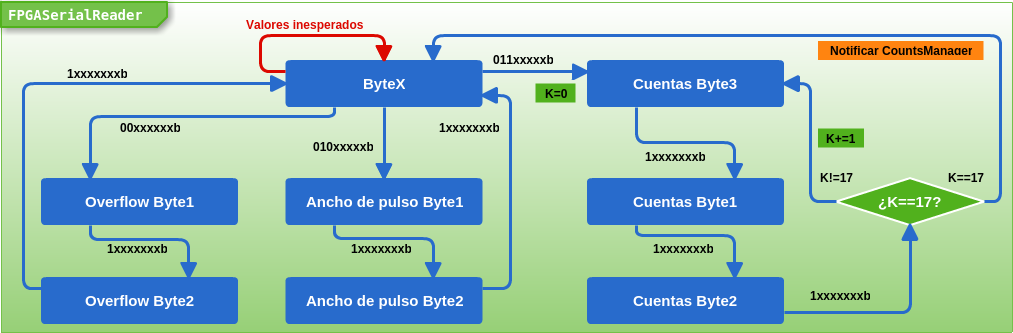
\includegraphics[keepaspectratio, width=1\textwidth]{./img/reader.png}
            \caption{Máquina de Moore. \texttt{FPGASerialReader}.}   
            \label{fig:reader}
        \end{figure}


    \section{\texttt{CountsManager}}
        Este módulo software se encarga de recolectar la información que el
        \texttt{FPGASerialReader} y \texttt{SensorsManager} generan.
        Seguidamente procede a calcular el valor global y las correcciones por
        presión y efficiencia. Finalmente se encarga de guardar los datos en la
        base de datos local. En la figura \ref{fig:soft_adquisición} podemos
        ver el diagrama que describe el funcionamineto que acabamos de
        explicar. A continuación procedemos a explicar a fondo estos pasos.
        \subsection{Recolectar información}
            Como vimos en el capítulo \ref{cap2}, la FPGA tan sólo
            transmite los datos de las cuentas cuando estas son solicitadas con
            el comando apropiado. Este módulo es el encargado de mandar el
            comando al principio de cada minuto. La información transmitida por
            la FPGA es procesada por el \texttt{FPGASerialReader} y almacenada
            en variables compartidas accesibles por el \texttt{CountsManager}.
            Después de mandar el comando apropiado para solicitar las cuentas
            este \emph{thread} se queda esperando hasta que el
            \texttt{FPGASerialReader} le notifique que las cuentas han sido
            enviadas y procesadas. Al ser notificado este módulo procede a leer
            de las variables compartidas donde está almacenada la información
            de las cuentas. Dicha notificación se realiza mediante un
            \texttt{threading.Lock}
            \par
            Los valores de presión atmosférica, diferencia de potencial generado por las fuentes de alimentación y temperatura ambiente son
            obtenidos haciendo uso del \texttt{SensorsManager}, que será descrito en secciones futuras de este capítulo.
        \subsection{Median Algorithm y Correcciones}
            Como hemos comentado al principio de esta sección este módulo
            calcula el valor global y una serie de correcciones sobre este. El
            valor global es una representación de las mediciones de todos los
            tubos, algo como una media. En el capítulo \ref{cap1} explicamos la
            necesidad de este valor, en este vamos a explicar el algoritmo que
            es utilizado para calcularle.
            \par 
            El MedianAlgorithm\cite{MedianAlgr} tiene dos entradas, un vector
            con las cuentas actuales de cada canal y un segundo vector con la
            media de cuentas para cada canal. Este vector con cuentas medias es
            calculado durante un intervalo temporal en el que la presión
            atmosférica no fluctúa y además esta se corresponde al valor medio
            de presión para la estación. Además es deseable que durante dicho
            intervalo no ocurran eventos que pueden afectar la cantidad de
            partículas que llegan al instrumento. Este vector de valores medio
            es especificado  en el archivo de configuración que previamente
            discutimos por lo que es fácilmente modificable. El algoritmo
            empieza calculando la desviación relativa sobre la media de cada
            canal, los canales con una desviación grande son descartados.
            Comparando la desviación de los canales restantes seleccionamos el
            mediano, de aquí el nombre del algoritmo. La desviación relativa
            del canal seleccionado es multiplicada por el sumatorio del vector
            de cuentas medias. El algoritmo devuelve el valor generado por la
            multiplicación. A continuación presentamos la implementación del
            algoritmo.
            \begin{lstlisting}[style=myPython]
def medianAlgorithm(self, counts):
   # Calculamos la desviación sobre la media.
   r=[x/z for x,z in zip(counts, self.channel_avg) 
      # Descartamos los canales con desviación grande.
      if z>0 and (x/z)>0.3 and (x/z)<10]
   tet = numpy.median(r)
   s0  = sum(self.channel_avg)
   return s0*tet
            \end{lstlisting}
            \par 
            Una vez calculado el valor global usando el MedianAlgorithm
            procedemos a calcular las dos correcciones. La primera es la
            corrección por presión. Como explicamos en el cápitulo \ref{cap1}
            la presión atmosférica influye en el proceso de adquisición. Para
            realizar la corrección por presión hay dos factores que se toman en
            cuenta. El primero es la desviación de la presión actual respecto
            al valor medio de presión para la estación. El segundo es el
            coeficiente de correlación de los tubos respecto a la presión
            atmosférica. Este coeficiente ha sido calculado por el equipo de
            CaLMa, siendo el método utilizado desconocido para el autor de este
            trabajo. En la ecuación \ref{eq:pression} podemos ver como se usan
            estos dos factores, donde $N_0$ es el valor sin corregir, $N$ el
            valor corregido, $\beta$ el coeficiente de corelación, $P$ la
            presión actual y $P_0$ la presión media para la estación.
            \begin{equation}\label{eq:pression}
              N=N_0*exp(\beta*(P-P_0))
            \end{equation}
            La segunda corrección que realizaremos es la corrección por
            eficiencia. Esta es una corrección muy simple, consiste en aplicar
            un factor multiplicativo a la corrección por presión. Esta
            corrección se puede ver en la fórmula \ref{eq:efficiencia}, donde
            $N_0$ es el valor de la corrección por presión, $N$ el valor de la
            corrección por eficiencia y $\gamma$ el factor de corrección. 
            \begin{equation}\label{eq:efficiencia}
              N=N_0*\gamma
            \end{equation}
            Cambios en el entorno de la estación pueden causar cambios en la
            cantidad de eventos medidos, por ejemplo las precipitaciones de
            nieve pueden reducir la cantidad de partículas que llegan al
            instrumento. Una persona que analiza los datos con propósito
            científico puede equívocamente asociar el decremento con algún
            fenómeno físico, mientras que este es debido a un fenómeno técnico.
            Este problema es solventado con la corrección por eficiencia.   
        \subsection{Base de datos}
            Como ya hemos explicado los datos son guardados en una base de
            datos para cuya gestión utilizamos \emph{Sqlite3}. En la base de
            datos tenemos tres tablas que a continuación procedemos a explicar.
                \par
            La primera tiene el nombre de \texttt{binTable}, nombre que hemos
            heredado de los primeros sistemas de adquisición rusos. En esta
            guardamos la información de las cuentas de cada minuto. Junto a las
            cuentas guardamos la fecha y hora en los que se realizó la medida,
            la lectura del barómetro y la lectura de las fuentes de alta
            tensión.
                \par 
            En la segunda tabla llamada \texttt{CALM\_ori}, nombre definido por
            el NMDB, guardamos el valor global y sus correcciones. Junto a
            estos valores también guardamos el valor de la fecha y hora en los
            que se realizó la medida, y también el valor de la presión
            atmosférica.
                \par
            En la última tabla guardamos los valores de los anchos de pulsos.
            Dado al gran número de pulsos, guardar la información de cada uno
            por separado no es práctico. Para ilustrar el problema pondremos de
            ejemplo la estación de CaLMa donde son procesados unos 4500 pulsos
            cada minuto, siendo esta una de las estaciones con menos eventos
            por minuto debido a su baja latitud. Para sobrevenir este problema
            construimos un histograma que guardamos en la base de datos, en
            forma de cadenas JSON\cite{JSON}. Los histogramas se construyen con
            los datos de diez minutos, intervalo que marca la resolución de los
            datos de esta tabla.

    \section{\texttt{DBUpdater}}
        Este módulo software es el encargado de actualizar el contenido de la
        base de datos remota. El funcionamiento de este es muy simple y se
        puede ver en la figura \ref{fig:soft_adquisición}. Empieza
        estableciendo la conexión con la base de datos remota. Si esta se
        establece se procede a leer la última entrada en la base de datos
        remota. Seguidamente el software calcula la diferencia entre las dos
        bases de datos, para este propósito usa la fecha y hora de la entrada
        leída de la base de datos remota. Finalmente el software selecciona las
        diferencias entre las dos bases de datos y las escribe en la remota. Es
        entonces cuando la ejecución de este \emph{thread} termina.  A fin de
        asegurar la sincronización en tiempo real se crea y lanza una instancia
        de este \emph{thread} cada minuto.
        \par
        Si la conexión con la máquina que alberga a la base de datos remota se
        pierde por un tiempo, cuando esta vuelva a restablecerse el
        \texttt{DBUpdater} sincronizará las dos bases de datos. Eventualmente
        si las diferencias entre las dos bases de datos son muy grandes la
        sincronización no ocurre de golpe, de esta manera evitamos sobrecargar
        al sistema.

    \section{\texttt{SensorsManager}}
        Este es el módulo software encargado de manejar los sensores. Por
        sensores nos referimos al barómetro, las fuentes de alta tensión o los
        termómetros si están presentes. A este módulo se le pasa la información
        referente a los sensores desde el archivo de configuración. De acuerdo
        con esta información este módulo invoca las funciones de configuración
        necesarias. Una vez realizada esta configuración inicial podemos
        empezar a leer la información de los sensores. Para este propósito este
        módulo exporta tres funciones, que se explican a continuación.
        \subsection{Presión atmosférica}
            Para leer el valor actual de la presión atmosférica este módulo nos
            ofrece la función \texttt{read\_pressure}. Si en el archivo de
            configuración hemos especificado que no tenemos barómetro esta
            función devuelve un \emph{-1}, así como en el caso de que se
            produzca algún error. Actualmente se soportan dos tipos de
            barómetros, el \emph{BM35} y el \emph{AP1}. La lógica para manejar
            estos dos barómetros se encuentra en los archivos
            \texttt{BM53Driver} y \texttt{AP1Driver} respectivamente. No
            explicaremos a fondo el funcionamiento de estos dos. Tan solo
            destacaremos que el \emph{BM35} se comunica mediante un puerto
            serie y el \emph{AP1} mediante tres señales digitales que son
            reloj, \emph{strobe} y datos.
        \subsection{Fuentes de alta tensión}
            En el caso de las fuentes de alta tensión las tenemos de dos tipos,
            analógicas y digitales. Las digitales transmiten su información
            mediante un puerto serie. Las analógicas mediante una señal
            analógica entre 0V y 5V, que es proporcional a la tensión ofrecida
            por la fuente. La lógica para operar con las fuentes analógicas
            está en el archivo \texttt{HVPSDriver}, la lógica para las fuentes
            digitales no está implementada porque no hemos podido trabajar con
            estas. Eventualmente si se produce algún error se devuelve el valor
            de \emph{-1}.
        \subsection{Temperatura}
            Como hemos comentado en muchas estaciones la temperatura ambiente
            es monitorizada también. Este no es el caso de CaLMa, razón por la
            que no hemos escrito ningunos drivers. Sin embargo el código está
            pensado para poder ser fácilmente ampliado en caso de necesidad.
